\subsubsection{SMOKE}
SMOKE\cite{Fan2019}-ի ալգորիթմը կազմված է երկու հիմնական փուլերից՝ բարձր ճշտության և մասշտաբայնության հասնելու համար։
Առաջին փուլում այն օգտագործում է պարզ, բայց ոչ ճշգրիտ վերլուծություն՝ հիշողության արտահոսքի բոլոր հնարավոր ուղիները
հայտնաբերելու համար և զտում է այն ուղիները, որոնք չեն կարող հանգեցնել արտահոսքի: Այս նպատակով նախ օգտագործվում է նոսր
արժեքների կախվածության գրաֆը, ապա կառուցվում է օգտագործման կախվածության գրաֆը(UFG): UFG-ն պարունակում է վերլուծության
համար բավարար ինֆորմացիա բոլոր դինամիկ հիշողության օբյեկտների մասին։ UFG-ի յուրաքանչյուր կող համապատասխանեցվում է պայմանների հետ,
որոնցից կախված ուղղորդվում է ծրագրի աշխատանքի ընթացքը։
Նկար \ref{fig:figure1}-ում(վերցված է\cite{Fan2019}-ից) պատկերված է UFG-ի օրինակ։ UFG-ն բացահայտ նկարագրում է ցուցիչի արժեքների հնարավոր
ընթացքն ստեղծելով սահմաններից դուրս գտնվող գագաթ(p@s8)։ Դա նշանակում է, որ դինամիկ հիշողության օբյեկտը, որն
օգտագործվում էր վերը նշված ցուցիչի միջոցով այլևս հասցեավորված չէ։

\begin{figure}[h]
    \centering
    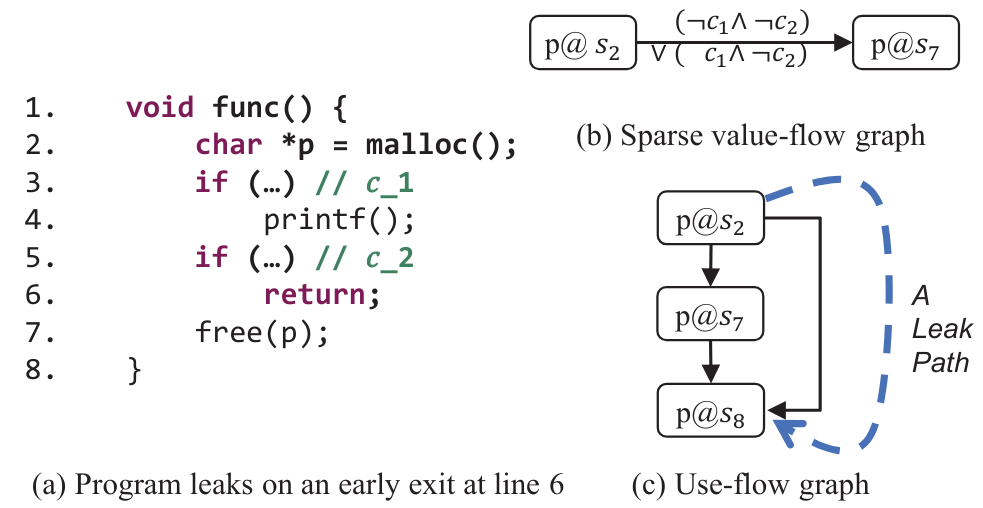
\includegraphics[width=0.6\textwidth]{pic1}
    \caption{Դինամիկ հիշողության արտահոսքի օրինակ}
    \label{fig:figure1}
\end{figure}

Երկրորդ փուլում այն օգտագործում է արդեն ստացված UFG-ի առավել ճշգրիտ վերլուծություն։ Սկզբում որոնում է բոլոր
ճանապարհները, որոնք չեն պարունակում դինամիկ հիշողություն օգտագործող օպերացիաներ։ Այնուհետև հայտնաբերված յուրաքանչյուր
ճանապարհի համար կիրառում է Z3 գործիքը\cite{Z3}՝ նրանց իրագործելիությունը ստուգելու համար: Այս գործընթացն անհրաժեշտ է
ճանապարհների զգայունությունն ապահովելու և կեղծ հայտնաբերված արտահոսքերը զտելու համար։ Գործիքն ունի որոշ սահմանափակումներ՝
\begin{enumerate}[itemsep=1mm]
    \item Վերլուծությունն արվում է դաշտերի հանդեպ ոչ զգայուն։
    \item Ցուցիչների վերլուծությունը ճշգրիտ չէ։
    \item Որոշ ճանապարհներ անիրագործելի են բարդ թվաբանական և միջֆունկցիոնալ տվյալների կախվածությունների պատճառով։
    \item Հաշվի չի առնվում թվաբանական գործողությունները ցուցիչների հետ, free(p + y) արտահայտությունը համարժեք է համարվում free(p)-ին, ինչն ակնհայտ սխալ է։
    \item Հաշվի են առվում միայն այն դեպքերը, երբ դինամիկ հիշողության առանձնացման գործողությունը բարեհաջող է անցնում։
\end{enumerate}

SMOKE-ը ծրագրավորված է LLVM-ի վերին մակարդակում և միայն բինար տարբերակն է հասանելի\cite{SMOKE}:
